\section{Proposed System}
The proposed Digital Logic Suite is a modular, extensible CLI application written in C++. It supports parsing Boolean expressions, generating truth tables, Karnaugh map minimization, circuit simulation, and Graphviz-based visualization. The system is designed for ease of use, extensibility, and integration into academic workflows.

\subsection{Description}
The suite consists of several core modules:
\begin{itemize}
    \item \textbf{CLI Module:} Handles user input, command parsing, and help documentation.
    \item \textbf{Expression Parser:} Parses and evaluates Boolean expressions using recursive descent or shunting yard algorithms.
    \item \textbf{Truth Table Generator:} Produces truth tables for given expressions.
    \item \textbf{Karnaugh Map Minimizer:} Simplifies Boolean expressions using K-map techniques.
    \item \textbf{Circuit Simulator:} Simulates logic circuits based on parsed expressions.
    \item \textbf{Graphviz Visualizer:} Generates .dot files and invokes Graphviz to visualize logic circuits and truth tables.
\end{itemize}
The suite is implemented using C++ OOP concepts, with each module encapsulated as a class or set of classes.


\subsection{System Block Diagram}
\begin{figure}[ht!]
    \centering
    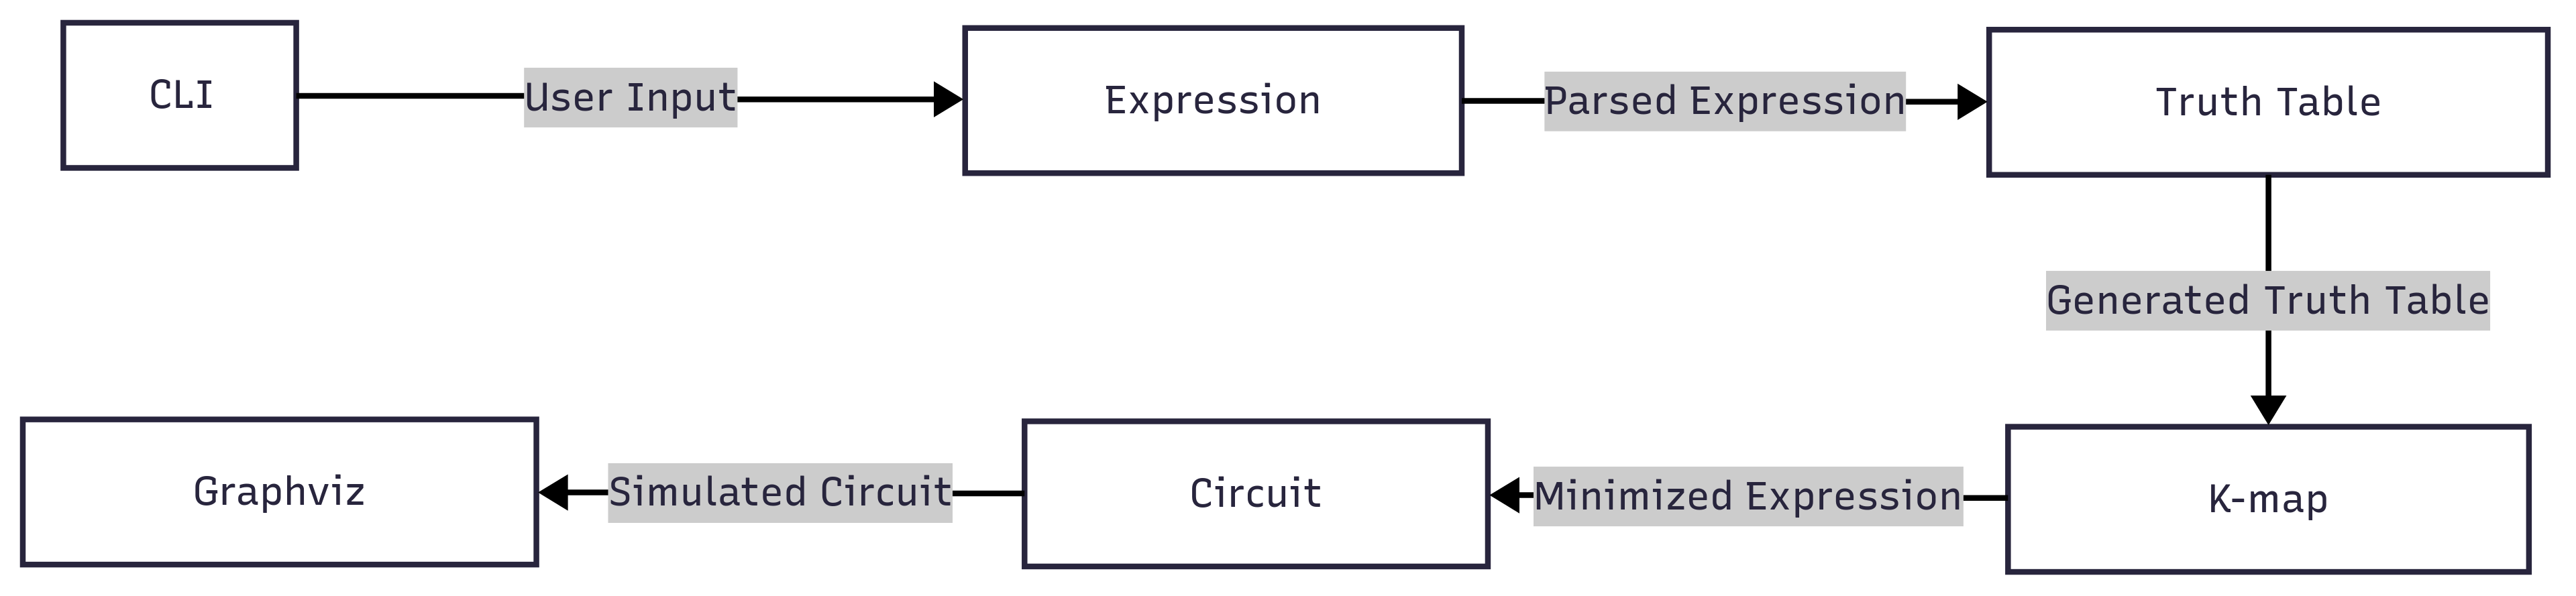
\includegraphics[width=0.9\textwidth]{images/inverted_C.png}
    \caption{System Block Diagram: CLI $\rightarrow$ Expression Parser $\rightarrow$ Truth Table Generator $\rightarrow$ Circuit Simulator $\rightarrow$ Graphviz Visualizer}
    \label{fig:system_block_diagram}
\end{figure}